\section{ShinyApp}\label{Sec:shiny}

\texttt{shiny} is an \texttt{R} package that allows the user to write interactive web applications. These are especially helpful when delivering information to people with no coding experience in a very user-friedly way.
\\
As described in the official site of \texttt{shiny}, in its most basic version an App is contained in a single script called \textit{app.R}. As the Apps become more and more complicated one can write the code in two scripts, \textit{ui.R} and \textit{server.R}, or even further split these into thematic scripts.
\\
The App structure is divided into two main elements:
\begin{itemize}
    \item \textit{ui}: The user interface object determines the appearance of the App itself. Here the possible inputs and the ouputs will be defined.
    \item \textit{server}: The server function uses the input values chosen in the App to produce the outputs indicated in the user interface. 
\end{itemize}

Finally the App will be called using the function \texttt{shinyApp(ui, server)}.
\\
A simple example from the \texttt{shiny} website shows this in action.

\begin{lstlisting}[language = R]
ui = fluidPage(
    titlePanel("Hello Shiny!"),
    sidebarLayout(
      sidebarPanel(sliderInput(inputId = "bins",
                               label = "Number of bins:",
                               min = 1, max = 50, value = 30)),
      mainPanel(plotOutput(outputId = "distPlot")))
)

server = function(input, output) {
    output$distPlot = renderPlot({
      x    = faithful$waiting
      bins = seq(min(x), max(x), length.out = input$bins + 1)
      hist(x, breaks = bins, col = "#75AADB", border = "white",
           xlab = "Waiting time to next eruption (in mins)",
           main = "Histogram of waiting times")})
}

shinyApp(ui = ui, server = server)
\end{lstlisting}

This simple App produces the result in figure \ref{figure:shiny_example}.

\begin{figure}[H]
\begin{center}
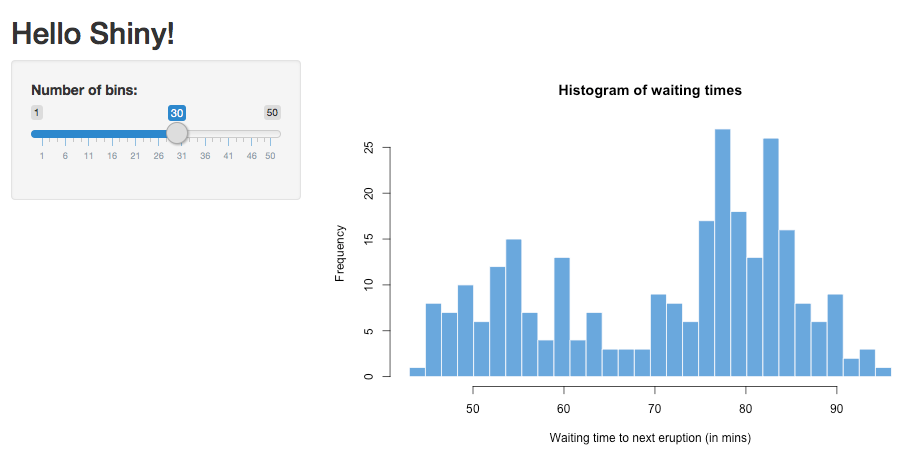
\includegraphics[width=0.6\textwidth, keepaspectratio]{shiny_example.png} \\
\caption{Example of simple ShinyApp from website}
\label{figure:shiny_example}
\end{center}
\end{figure}

Because of its interactiveness and flexibility a ShinyApp was built for this project in order to enable the final user a chance to a first hand analysis of the data. The App is reachable at this link (INSERT SHINY APP LINK).
